\chapter{Lenses}

Lenses are optical devices with perfect or approximate axial symmetry
that transmit and refract light, converging or diverging the
beam. There are two main types of lenses, distinguished by their shape
and the way they refract light:\index{lenses}

\begin{itemize}
    \item \textbf{Converging (or Convex) Lenses:} These are thicker at
      the center than at the edges. When parallel light rays enter a
      convex lens, they converge to a point called the focal
      point. Examples of converging lenses include magnifying glasses
      and camera lenses.

      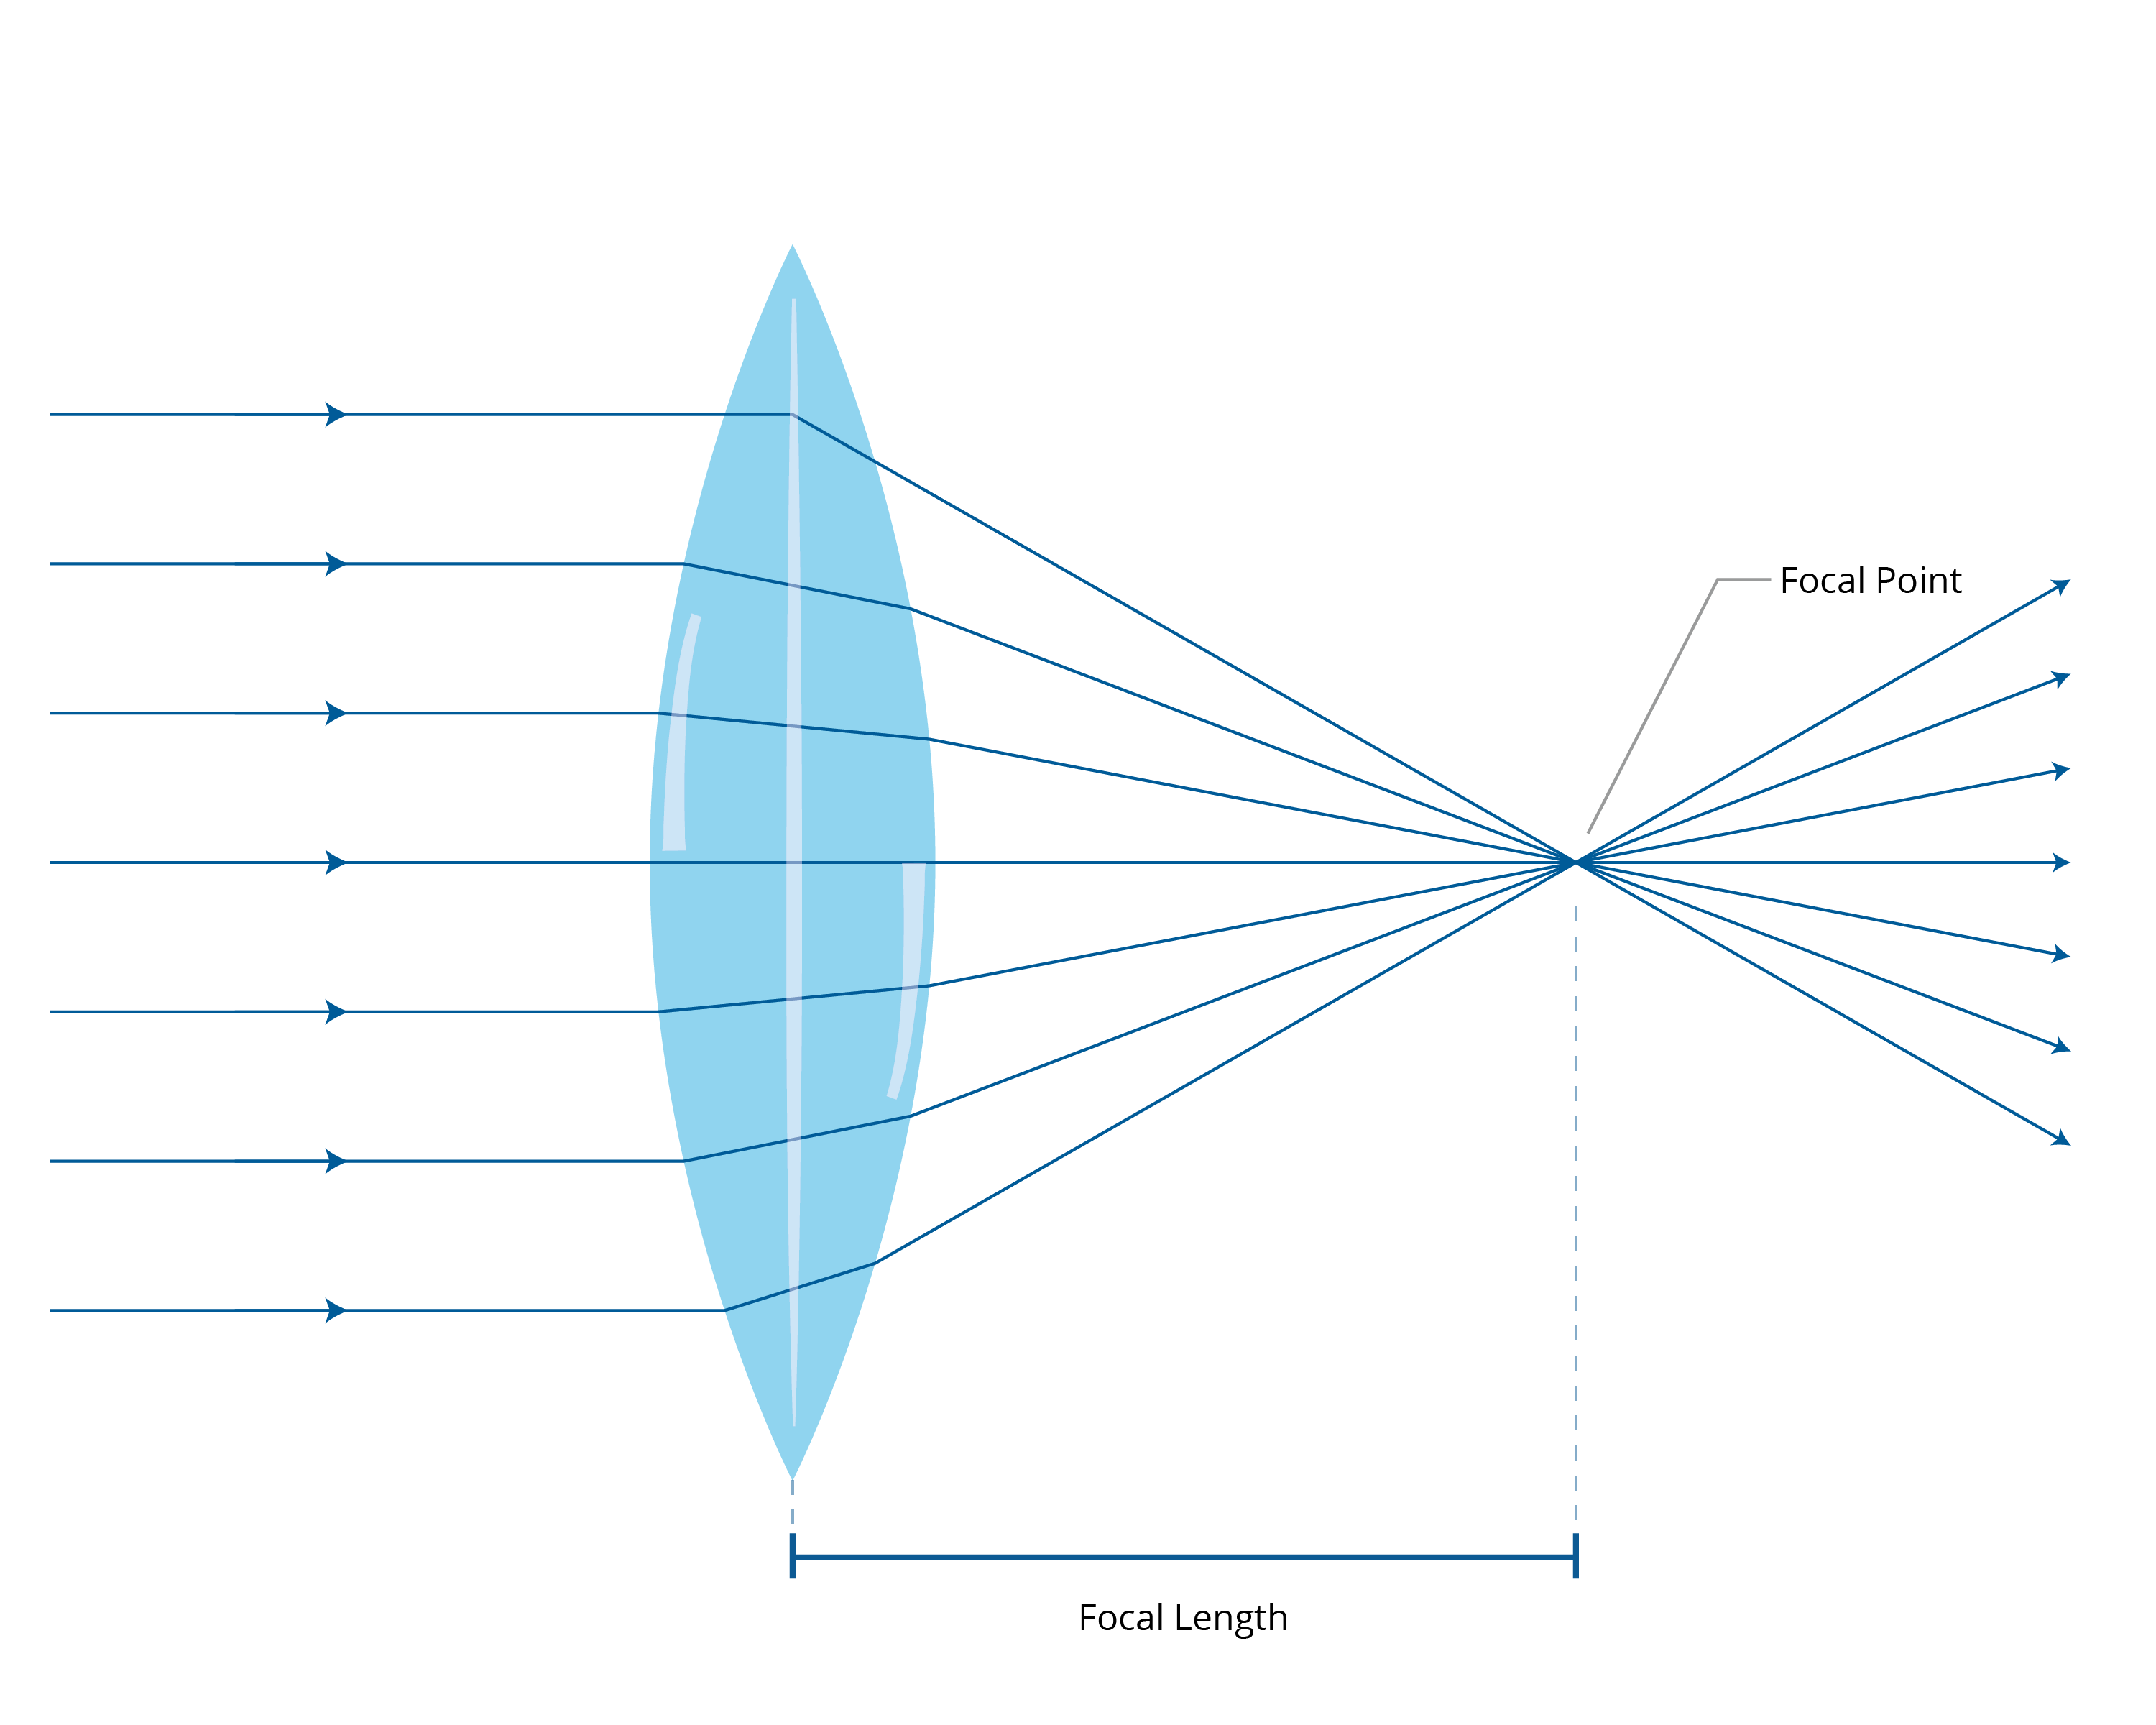
\includegraphics[width=0.5\textwidth]{convex.png}

    \item \textbf{Diverging (or Concave) Lenses:} These are thinner at
      the center than at the edges. When parallel light rays enter a
      concave lens, they diverge or spread out. These lenses are often
      used in glasses to correct nearsightedness.
      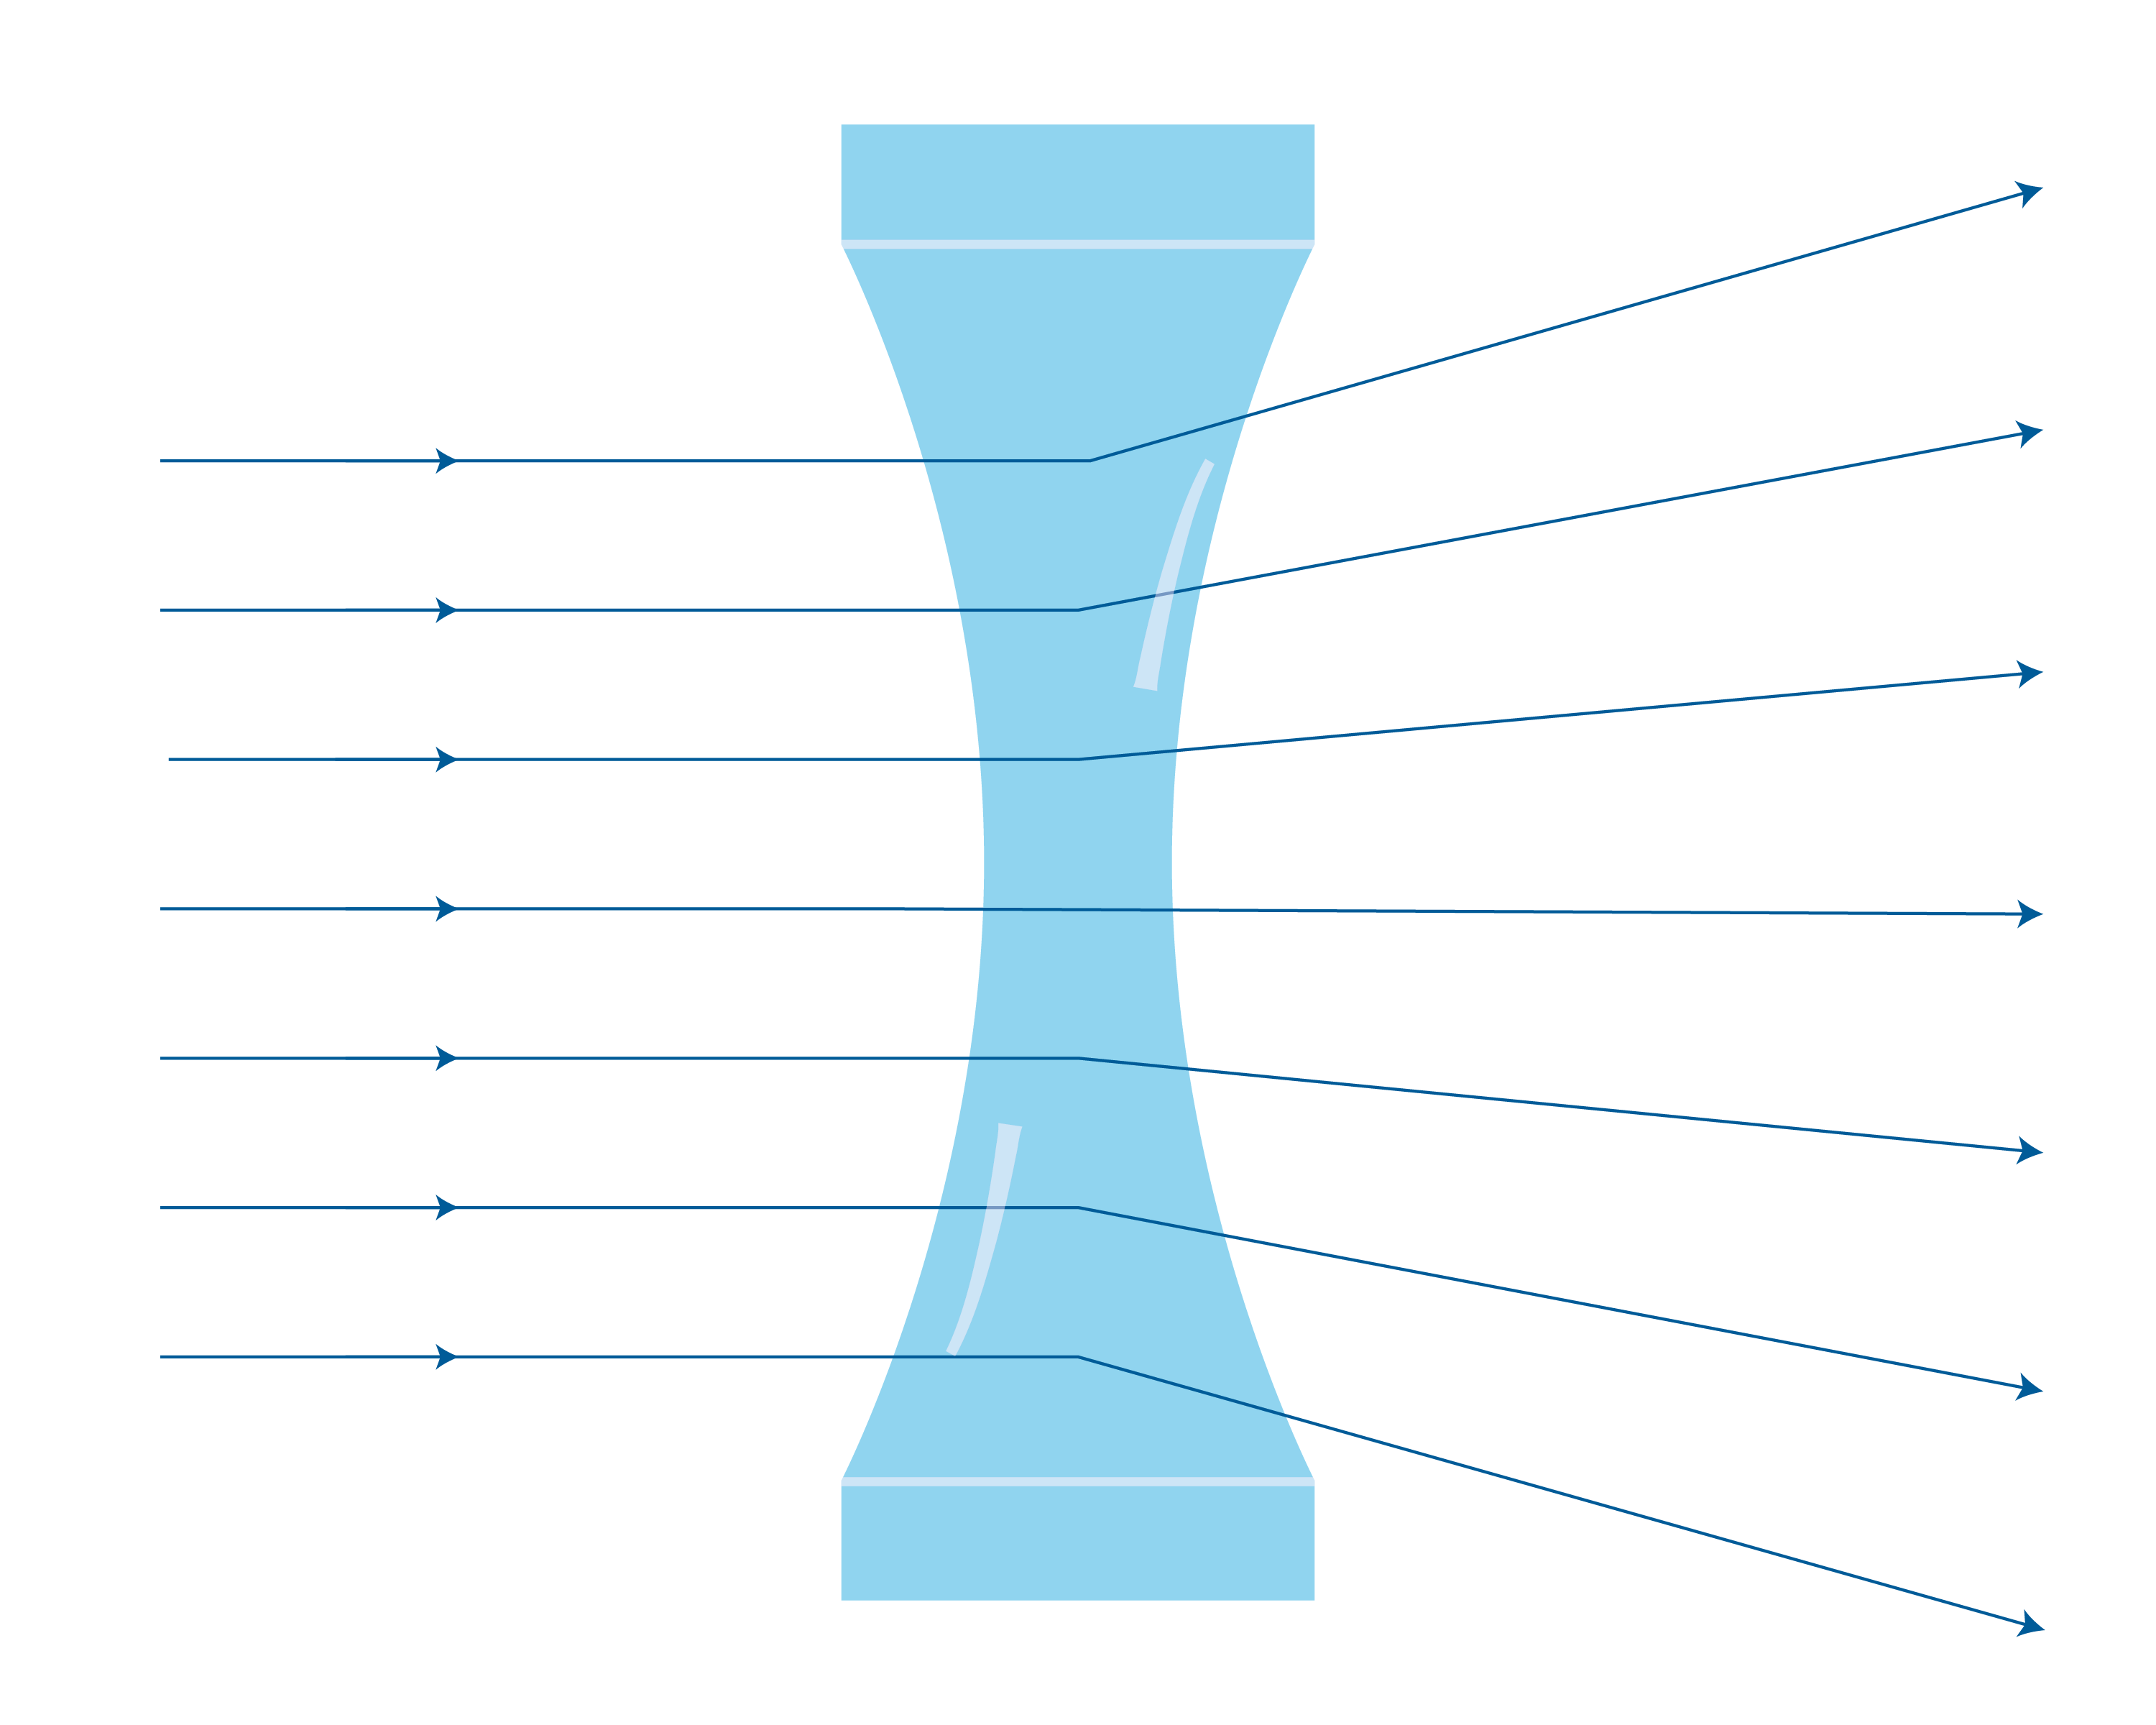
\includegraphics[width=0.5\textwidth]{concave.png}

\end{itemize}

\section{Focal Length}

The focal length of a lens is the distance between the center of the
lens and the focal point. It is determined by the lens shape and the
refractive index of the lens material. For a converging lens, the
focal length is positive, and for a diverging lens, the focal length
is negative.\index{focal length}

\section{Refractive Index}

The refractive index of a material is a measure of how much the speed
of light is reduced inside the material. The refractive index $n$ of a
material is given by the ratio of the speed of light in a vacuum $c$
to the speed of light $v$ in the material:\index{refractive index}

\[
n = \frac{c}{v}
\]

The refractive index affects how much a light ray changes direction,
or refracts, when entering the material at an angle. A higher
refractive index indicates that light travels slower in that medium
and the light ray will bend more towards the normal.

Lenses work by refracting light at their two surfaces. By choosing the
right lens shape and material, lenses can be designed to bring light
to a focus, spread it out, or perform more complex transformations.
